%!TEX root = bambi-thesis.tex



In this introduction it is first briefly described the motivation, objective and scope of the project this thesis has been developed in. Once the background has been well set and explained, this written work will elaborate in details the specific subject of \textit{georeferencing an agricultural field} and \textit{Coverage Path Planning}.

\section{Bambi Project} % (fold)
\label{sec:bambi_project}
Bambi Project aims to make the coverage flight over agricultural fields completely automatic for the purpose of wildlife rescuing.
% section bambi_project (end)
\subsection{Motivation} % (fold)
\label{ssec:motivation}
 Deers gives birth to their offspring during April and May \cite{MowlingMortality}, often choosing meadows as they consider it a safe spot. This period is unfortunately the same in which meadows are cut. The results is that every year a great number of young deers fall victim of combine harvesters cutting hay. Germany counts about 100000 death every harvest season \cite{MowlingMortality}.\par
 It is, as a matter of fact, difficult to locate small animals hidden in vast grasslands especially if they freeze when they feel under threat. For this specific reason the proposal design is based on an \acrfull{uav}\cite{ICAO} and more precisely a quad-copter equipped with a thermal camera.
 An aerial vehicle is able to efficiently cover large surfaces way faster then any other ground alternatives and guarantees the best viewpoint for the specific kind of wildlife research. Moreover, it has been chosen a copter rather than a fixed wing model for its holonomic properties which turns out to be very useful in upland regions as well as for small and irregular fields. It is basically why in search and rescue operations helicopters are often adopted instead of planes.

\subsection{Importance for Wildlife and for Agricultural}
\index{Agriculture}
In early hunting literature from as far back as the mid-19th century, references can be found to significant losses of breeding partridges and pheasants from the use of sickle and scythe. Due to the fierce competition in the agricultural sector, developments in agricultural technology have brought about a tremendous acceleration in mowing techniques, with tendency still rising. Today, mowing speed can even exceed 15 km/h, while at the same time ever-wider mowers are used. Nesting birds, young hares and fawns are regular victims of such mowers and even full-grown wild animals cannot always escape.

\subsubsection{Affected Species} % (fold)
\label{ssub:affected_species}
Grassland is used by countless species of wildlife as food, cover and reproduction habitat. Apart from leverets, fawns and various field birds, small mammals, amphibians and insects all fall victim to the practice of early and more frequent mowing. Formerly reliable survival strategies proven successful over thousands of years have a devastating effect in mowing situations. The instinct of the brooding partridge hen to sit tight on her nest, or of the hare or fawn to freeze motionless, now prove fatal. The optimized patterns of predator avoidance behavior which wild animals have evolved can no longer keep up with the developments in modern cultivation techniques.
\begin{figure}[ht]
    \centering
    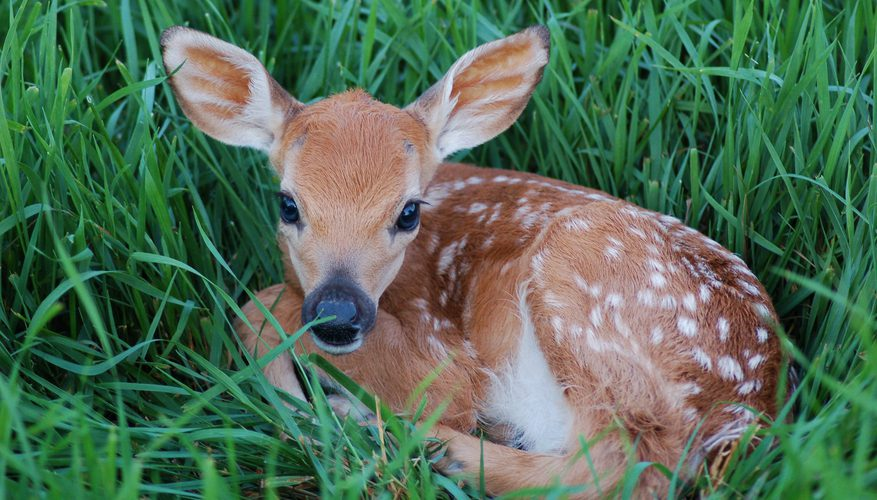
\includegraphics[width=0.6\textwidth]{figures/C1/fawns.jpeg}
    \caption{Fawn hiding in meadow}
    \label{fig:}
\end{figure}


% subsubsection affected_species (end)

\subsection{Measure to Reduce Wildlife Losses} % (fold)
\label{sub:measure_to_reduce_wildlife_losses}
 The most important factor influencing wildlife mortality is without doubt the time of mowing. On the other hand, economic considerations make this a crucial factor for the farmer, too. A late mowing is good for wildlife but not ideal for the farmer from the point of view of yield and quality. Yet there are some other factors in the mowing of arable land which offer potential for reducing wildlife losses \cite{MowlingMortality}:
\begin{itemize}
	\item \textit{Cutting height}: the higher the cut, the lower will be the losses suffered by crouching animals and nesting birds.
	\item \textit{Mowing direction}: mowing the field from the center outwards gives fully-grown wild animals the opportunity to escape.
	\item \textit{Mowing date}: late cuts,from mid-July onwards, reduce the losses to wildlife during the nesting and rearing period.
	\item \textit{Mowing strategy}: mowing of partial areas, leaving edge strips unmown.
	\item \textit{Mowing frequency}: a longer interval between first and second cuttings reduces the mortality rate, especially for ground-nesting birds.
	\item \textit{Mowing technology}: cutter-bar mowers cause less harm to wild animals than rotary mowers.
\end{itemize}
A practical approach which do not impact mowing strategy is the one adopted in a German wildlife rescue project consisting in deploying small aerial drones to find young deers hiding in tall grass.
% subsection measure_to_reduce_wildlife_losses (end)

\section{UAV Usage for Wildlife Research} % (fold)
\label{sec:state_of_the_art}
 During last years, the increasing interest and development of \acrfull{uav} makes them affordable and suitable for many different applications. Specifically, in wildlife research, drones are frequently use as they are less expensive, quieter, and safer than traditional manned aircraft. Most studies recorded minimal or no visible behavioral responses to \acrshort{uav}; however, \acrshort{uav} are capable of causing behavioral and physiological responses in wildlife when observing at close range. \cite{doi:10.1002/fee.1281}.\par
 For the case under-study, the "Flying Wildlife Finder", represents the state-of-the-art.
 The project, developed by the German Aerospace Center (DLR), is an application system which prevents accidents by detecting animals hidden in tall grass during the hay harvest. 
 The "Flying Wildlife Finder", a remotely controlled aerial drone equipped with sensors and a GPS link, is sent on a reconnaissance flight before mowing starts. A high resolution thermal imaging camera detects the temperature of animals hidden in the grass, which is higher than the ambient temperature of the field. Once the animal is located a search party is led to the fawn’s resting place with the help of GPS.
 This solution proves to be good as it is less time-consuming then using trained dog, while maintaining even higher "hit-rate", but it has the main drawback of requiring at least two specialists: one pilot and one camera operator that must be focused on the thermal video stream during the whole mission duration.

 

 \section{Proposal Solution} % (fold)
 \label{sec:proposal_solution}
 Bambi project consists in a standard \acrshort{uav} equipped with a thermal camera and an onboard computer.
 The mission is carried out by an operator and an assistant who is entitled to rescue the animal once it has been located.
 The vehicle automatically scan the entire field and inform the operator when thermal irregularity is detected sending the GPS position. At this point the rescuing team is guided toward the animal with the help of the thermal video signal. \\
 This procedure requires that the vehicle passes autonoumusly through the following steps:
 \begin{enumerate}
   \item Takeoff and flight to a position where having a complete view of the field so to shout a photo of the whole field.
   \item Generate a georeferenced photo of the field, identify the field boundary and store it as a geographic polygon (set of \acrshort{gps} coordinates).
   \item Calculate the \textit{coverage path}.
   \item Generate a \textit{timed dependent trajectory} taking into account dynamic constraints of the vehicle.
   \item Make the drone to follow the computed trajectory while avoiding obstacles.
   \item Interrupt the flight when the thermal camera sense a spot having an higher temperature with respect to the field and guide the user to the target location.
   \item When the field has been completely covered return to home position.
 \end{enumerate}
 % section proposal_solution (end)

 \subsection{Project Goals} % (fold)
 \label{sec:bambisaver_goals}
 The scope of the Bambi project is to ease a lot wildlife rescuing using \acrshort{uav} so that it can be handled also by untrained people. This must be guaranteed even in adverse environments, especially for uneven fields as it is in upland regions.
 Along with this, it is of particular interest to keep modularity in every hardware and software components. This is to permit easier implementation of new features or improvements to the existing ones.
 All this basic concepts have been used as guidelines during the design and implementation stages (e.g. the choice of \acrshort{ros} as framework for the whole software).

 \subsection{Software Architecture} % (fold)
 \label{sub:software_design}
 The raspberry Pi 3 it is used as on-board computer, it runs \acrshort{ros} (see appendix \ref{appendix:ros}) and manages the transition between the different mission's phases. The software develops according to the usual \acrshort{ros} philosophy \cite{288}, thus it is composed of six nodes implementing every mission component as an independent module. \autoref{fig:rqtgraph} displays all the nodes and their communication scheme. The \textsf{mission\_controller} node, in the center of the graph, handle all the mission procedures and timing implementing a FSM (\textit{Final State Machine}).
\begin{figure}[ht]
    \centering
    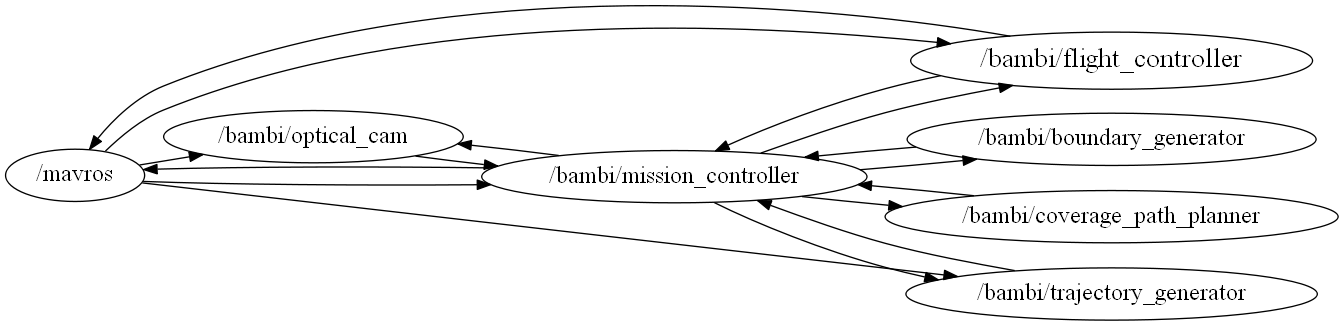
\includegraphics[width=1\textwidth, angle=0]{figures/C1/rqtgraph-all-noTopic.png}
    \caption{Nodes and Topics graph}
    \label{fig:rqtgraph}
\end{figure}\\
 In the following chapter the thesis will examine in particular two parts of the project:
 \begin{itemize}
  	\item \textit{Geo-referencing the mission's environment and get the field boundary}. This is of great importance, as it define the mission's range which is fundamental for every successive tasks.
  	\item \textit{Planning the coverage path}. It regards planning the geometric path so that the whole field of interest is covered by the sensor footprint.
  \end{itemize}
  % subsection software_design (end)

\section{Geo-referencing Mission's Environment} % (fold)
\label{sec:geo_referencing_mission_s_environment}
Chapter \ref{cha:georeferencing_the_mission_s_environment} develops the subject of Georeferencing the mission's environment dividing it into two different tasks: 
\begin{enumerate}
  \item Get an orthorectified photo of the workplace, thus an uniform scaled pictures of the field with the same lack of distortion as a map and having geo-position information encoded into it.
  \item Detect the field border and store it in a standard format that is commonly used to encode geographic features.
\end{enumerate}
In first place, it is explained what is orthorectification and the process to achieve it. Then free orthophoto database are presented with a special care for Google Imagery database and Google Earth application.
Google Earth provides a toolbox to trace path over the map. This is used to define the field boundary easily directly on the orthophoto and later to save it in \acrfull{kml}. The main features of \acrshort{kml} is therefore illustrated as well as how to handle it in Python scripts.

% section geo_referencing_mission_s_environment (end)

\section{Coverage Path Planning} % (fold)
\label{sec:coverage_path_planning}
In \autoref{cha:coverage_path_planning} the topic of \acrfull{cpp} is explained providing a basic knowledge of the existent approaches to the problem.\par
\acrlong{cpp} is the task of determining a path that passes over all points of an area or volume of interest while avoiding obstacles. This task is integral to many robotic applications, such as vacuum cleaning robots, painter robots, autonomous underwater vehicles creating image mosaics, demining robots, lawn mowers, automated harvesters, window cleaners and inspection of complex structures. That is why it is an important problem in \textit{mobile robot navigation} and even if the research about this issue developed rapidly, the governing algorithm to efficiently find the optimal path has not been found yet.
% section coverage_path_planning (end)
% % section innovation (end)